% ======================================================================
% CAPÍTULO 1: INTRODUCCIÓN
% ======================================================================

\chapter{Introducción}
\label{cap:introduccion}

\section{Contexto y Antecedentes}
\label{sec:intro_contexto}

Cualquier persona ha experimentado en algún momento de su vida la sensación de agotamiento tras una larga jornada de trabajo o esfuerzo prolongado. Sin embargo, en entornos profesionales de alta responsabilidad ---como la conducción de vehículos de transporte, la intervención quirúrgica en hospitales, el control del tráfico aéreo o la operación de maquinaria industrial pesada--- la fatiga no es un simple malestar pasajero: representa un deterioro inadvertido pero crítico de la capacidad de reacción y juicio que puede desembocar en accidentes graves o pérdidas humanas. En la era de la computación ubicua y los dispositivos inteligentes de uso cotidiano, surge una pregunta científica e ingenieril apasionante: ¿es posible detectar y predecir de forma objetiva, automática y no invasiva este estado de agotamiento fisiológico a partir de señales biométricas registradas por sensores vestibles antes de que se produzca una falla de seguridad?

Desde una perspectiva psicofisiológica formal, la fatiga no constituye un estado unívoco ni estático, sino un proceso dinámico de degradación progresiva de la capacidad funcional, derivado de la actividad sostenida en el tiempo, la privación de descanso o la sobrecarga psicofísica \cite{enoka2008muscle, grandjean1979fatigue}. En el ámbito de la ingeniería informática y las ciencias biomédicas, resulta indispensable delimitar con precisión la terminología empleada, distinguiendo formalmente entre cuatro conceptos estrechamente vinculados pero metodológicamente diferenciados:
\begin{itemize}
    \item \textbf{Fatiga Física (o Periférica/Muscular):} Se define como la reducción transitoria y reversible de la capacidad máxima de generación de fuerza o potencia mecánica de los grupos musculares tras un esfuerzo contráctil sostenido o repetitivo \cite{enoka2008muscle}. A nivel metabólico y sistémico, involucra el agotamiento de sustratos energéticos, la acumulación de metabolitos (como el lactato y protones $H^+$) y alteraciones en el acoplamiento excitación-contracción en las fibras musculares.
    \item \textbf{Fatiga Mental (o Central/Cognitiva):} Es un estado psicofisiológico inducido por la ejecución prolongada de tareas cognitivas exigentes, caracterizado por una sensación subjetiva de cansancio, disminución del estado de alerta, ralentización en los tiempos de reacción y un deterioro sensible en las funciones ejecutivas, tales como la memoria de trabajo, la atención sostenida y la flexibilidad cognitiva \cite{boksem2005effects}.
    \item \textbf{Somnolencia (\textit{Sleepiness}):} Hace referencia a la propensión, presión homeostática o necesidad biológica inminente hacia el sueño \cite{akerstedt1990subjective, hoddes1973quantification}, la cual, aunque interactúa con la fatiga mental, obedece a ritmos circadianos e historia previa de vigilia.
    \item \textbf{Fatigabilidad (\textit{Fatigability}):} Describe la tasa o velocidad a la que un individuo particular experimenta fatiga ante una carga de trabajo estandarizada, reflejando diferencias individuales intrínsecas en la tolerancia al esfuerzo \cite{kalanadhabhatta2021fatigueset}.
\end{itemize}

Históricamente, la cuantificación de la fatiga se ha sustentado de manera predominante en instrumentos de autoevaluación subjetiva mediante cuestionarios psicométricos estandarizados, tales como la Escala de Somnolencia de Stanford (SSS) \cite{hoddes1973quantification}, la Escala Visual Analógica (VAS), la escala de esfuerzo percibido de Borg o el índice NASA-TLX. Si bien estas escalas proporcionan una ventana directa a la percepción del usuario, presentan severas limitaciones metodológicas: adolecen de sesgos de memoria, susceptibilidad al estado anímico, baja resolución temporal y la necesidad imperativa de interrumpir la actividad del sujeto para su cumplimentación, lo que invalida su aplicabilidad en escenarios de monitorización continua en tiempo real. Para superar estas barreras mediante monitorización biomédica continua, en este trabajo se formula un estudio exhaustivo sustentado en una taxonomía integral de paradigmas computacionales (esquematizada en la Figura~\ref{fig:intro_taxonomia}).

\begin{figure}[H]
    \centering
    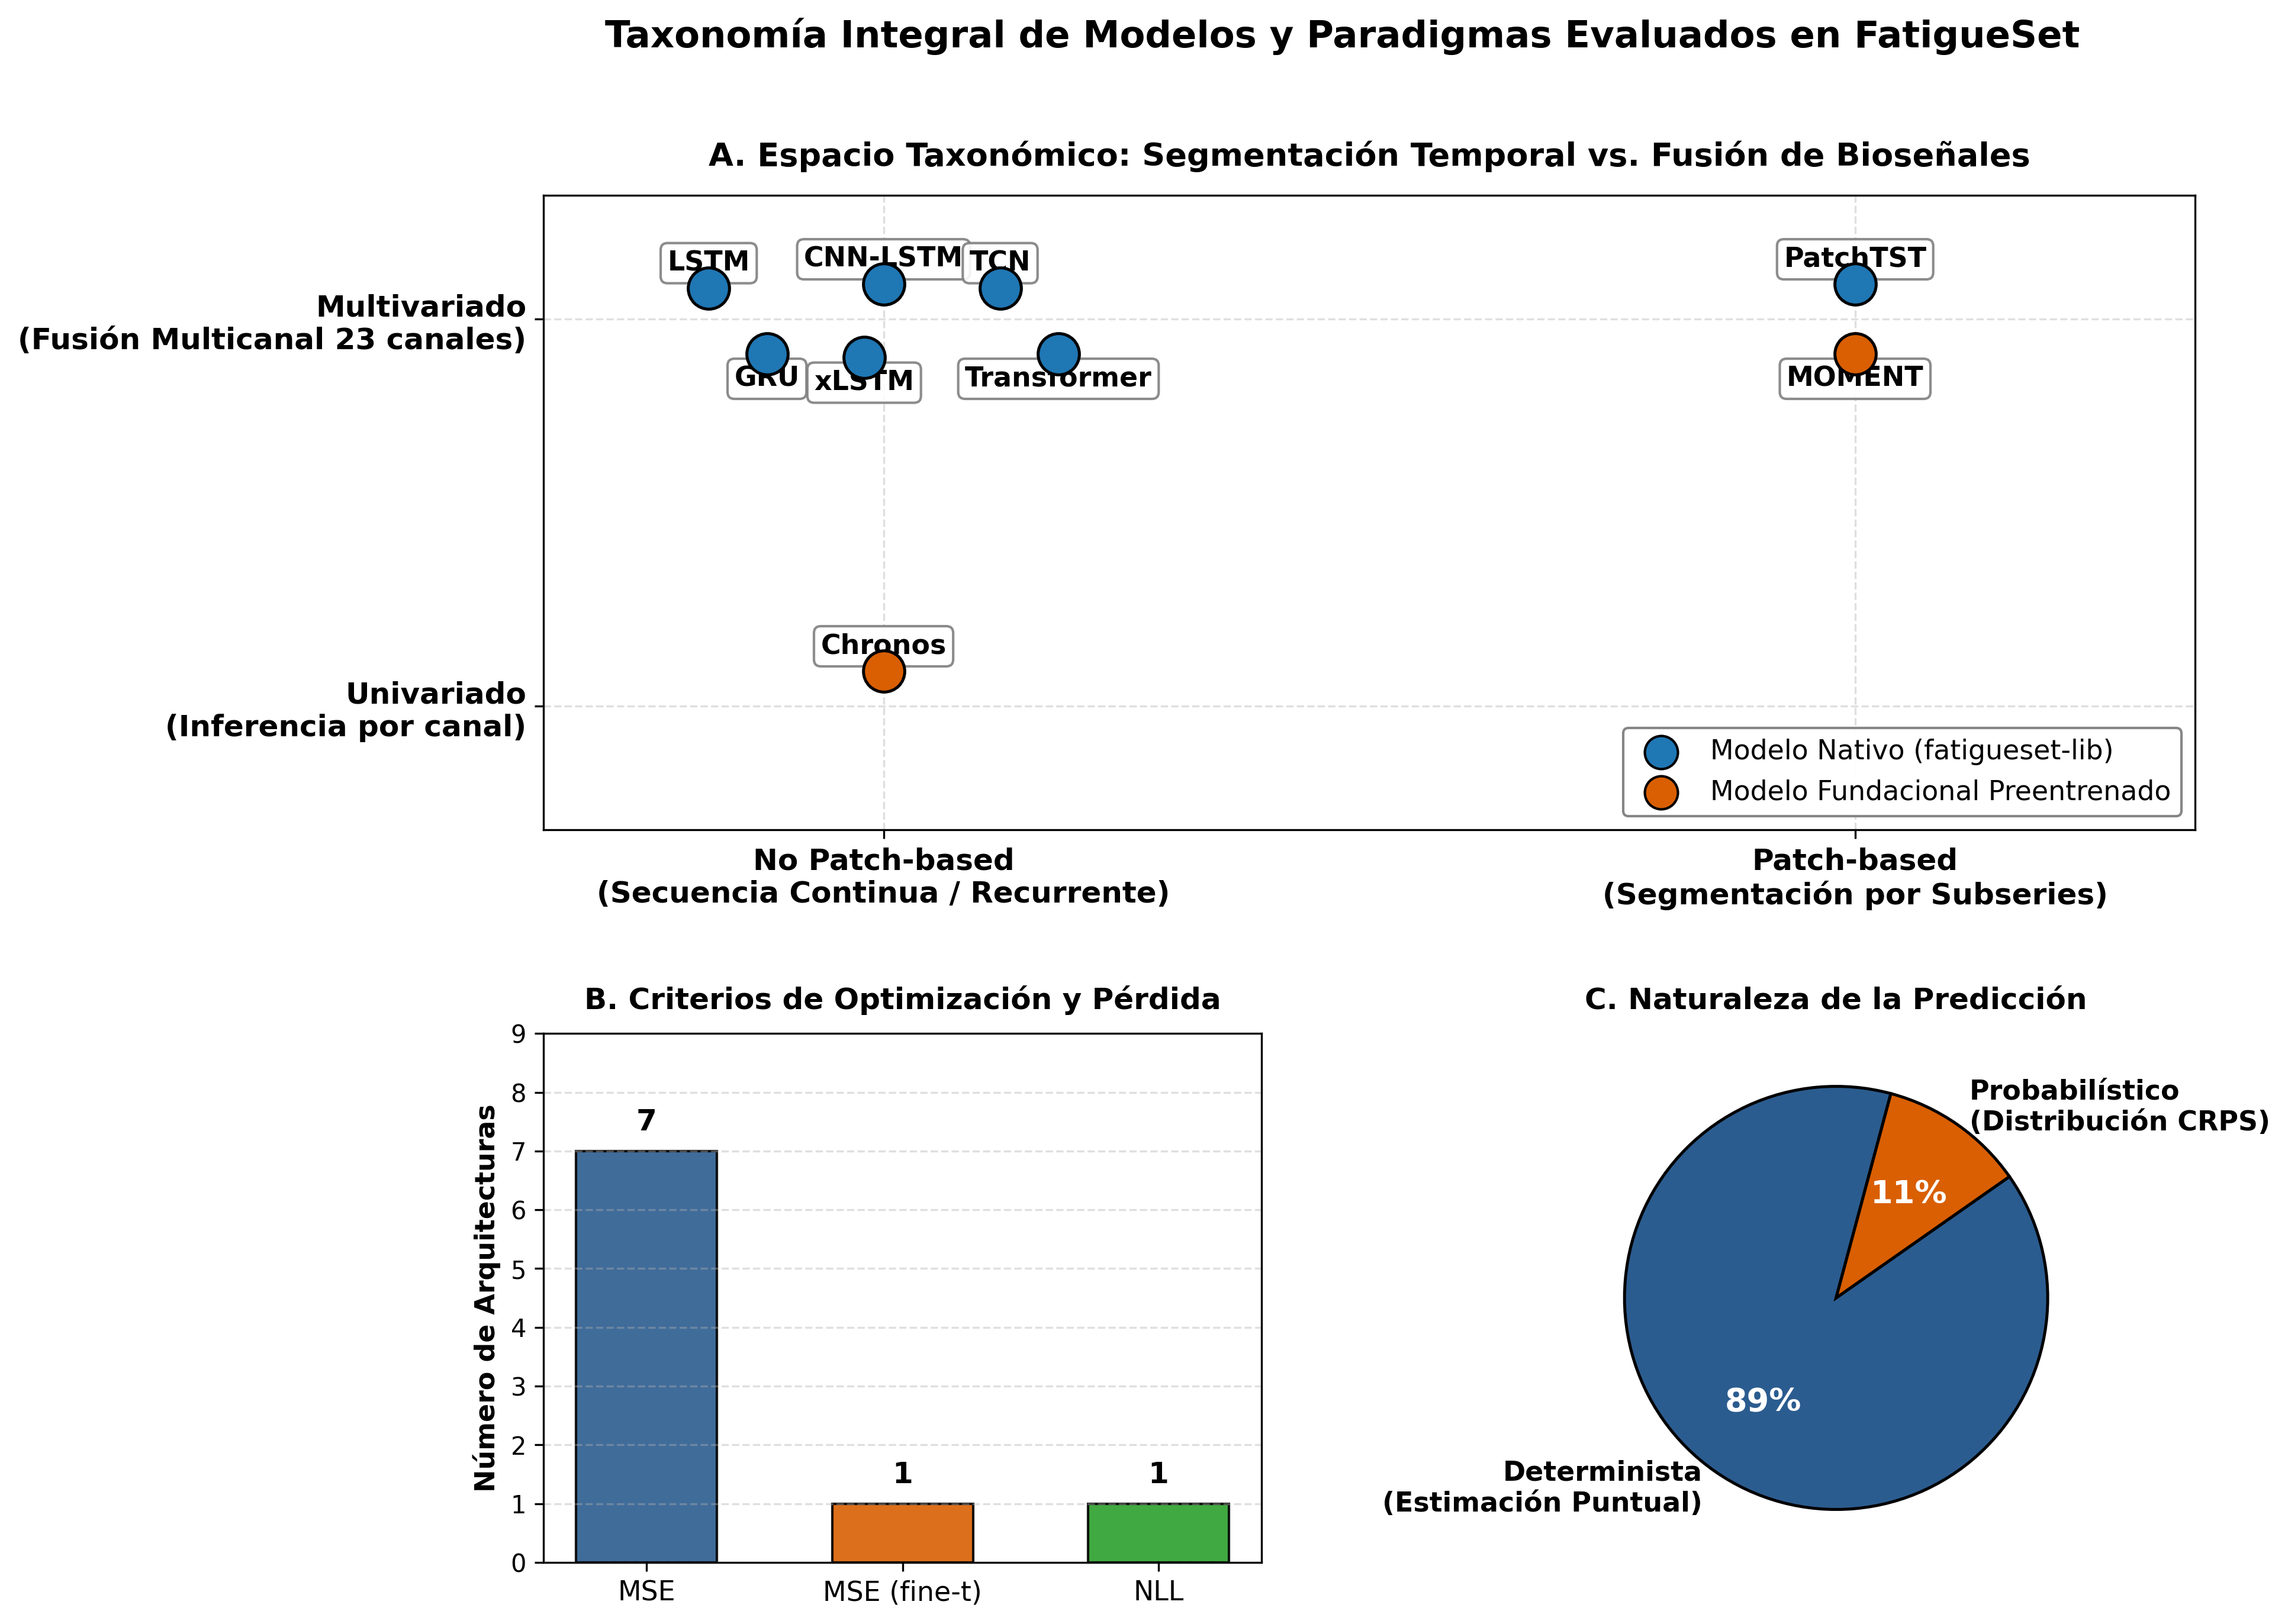
\includegraphics[width=0.86\textwidth]{figures/taxonomia_modelos_tfg.png}
    \caption{Taxonomía integral de modelos y paradigmas evaluados en este Trabajo de Fin de Grado: (A) espacio de segmentación temporal y fusión multicanal de bioseñales, (B) funciones de pérdida y criterios de optimización, y (C) naturaleza determinista frente a probabilística de la predicción. (Fuente: Elaboración propia).}
    \label{fig:intro_taxonomia}
\end{figure}

En la última década, la convergencia entre la microelectrónica de bajo consumo, la computación ubicua (\textit{ubiquitous computing}) y los sensores biomédicos no invasivos ha impulsado la proliferación de dispositivos vestibles (\textit{wearables}) de alta precisión \cite{kalanadhabhatta2022fatigueset}. Dispositivos comerciales como pulseras de fotopletismografía y conductancia cutánea (Empatica E4), bandas torácicas con electrocardiografía y monitorización respiratoria (Zephyr BioHarness 3.0), diademas de electroencefalografía (Muse S) y sensores intrauriculares (Nokia eSense) permiten registrar de forma ininterrumpida bioseñales complejas como:
\begin{enumerate}
    \item \textbf{Variabilidad de la Frecuencia Cardíaca (HRV):} Reflejo de la modulación autonómica simpática y parasimpática en el nódulo sinoauricular \cite{taskforce1996heart}.
    \item \textbf{Actividad Electrodérmica (EDA):} Indicador directo de la activación simpática periférica mediante la sudoración ecrina \cite{boucsein2012electrodermal}.
    \item \textbf{Ritmos Electroencefalográficos (EEG):} Oscilaciones neuroeléctricas corticales organizadas en bandas delta ($\delta$, 0.5--4 Hz), theta ($\theta$, 4--8 Hz), alfa ($\alpha$, 8--12 Hz), beta ($\beta$, 12--30 Hz) y gamma ($\gamma$, >30 Hz), cuyos ratios de potencia relativa correlacionan fuertemente con la carga mental y el decaimiento de la vigilia \cite{klimesch1999eeg}.
    \item \textbf{Patrones Respiratorios y Dinámica Cinemática:} Frecuencia respiratoria e índices de acelerometría triaxial que contextualizan la intensidad motora y la agitación corporal.
\end{enumerate}

No obstante, el modelado automático de estas señales plantea retos de enorme calado en el campo de la Ciencia de Datos y el Aprendizaje Automático: las series temporales fisiológicas son altamente no estacionarias, exhiben marcadas discrepancias en frecuencias de muestreo (desde 1 Hz hasta 256 Hz), contienen artefactos de movimiento y presentan una gran variabilidad inter-sujeto (dos individuos sometidos a la misma tarea cognitiva o física experimentan respuestas fisiológicas divergentes).

En este escenario, el conjunto de datos de referencia internacional \fatigueset{} \cite{kalanadhabhatta2021fatigueset}, publicado por investigadores de Nokia Bell Labs y la Universidad de Cambridge, constituye una plataforma experimental idónea y pionera. \fatigueset{} captura de forma sincronizada las señales de 12 sujetos a lo largo de múltiples sesiones experimentales estructuradas con protocolos rigurosos de fatiga física y mental, proveyendo un total de 23 canales fisiológicos continuos emparejados con evaluaciones cuantitativas de fatiga física y mental en escala continua (0--100).

\section{Motivación y Justificación}
\label{sec:intro_motivacion}

La necesidad de investigar y desarrollar sistemas capaces de predecir la fatiga de forma continua, objetiva y no invasiva está plenamente justificada desde múltiples perspectivas socioeconómicas, científicas, tecnológicas y metodológicas:

\begin{enumerate}[label=\bfseries M\arabic*.]
    \item \textbf{Seguridad Laboral y Prevención de Riesgos:} Según la Organización Internacional del Trabajo (OIT), una fracción sustancial de los accidentes de alta gravedad en sectores críticos ---como el transporte de pasajeros y mercancías, el control del tráfico aéreo, la minería, la construcción y las guardias médicas hospitalarias--- están directa o indirectamente vinculados al agotamiento físico o al colapso cognitivo por fatiga. Disponer de algoritmos predictivos capaces de alertar con antelación del inicio de la fatiga antes de que se produzca una pérdida crítica de reflejos salvaría miles de vidas al año y reduciría costes millonarios derivados de indemnizaciones y bajas laborales.
    \item \textbf{Salud Ocupacional y Ergonomía Digital:} El estrés crónico y la sobrecarga laboral en entornos de teletrabajo e interacción prolongada con pantallas generan fatiga mental crónica y síndrome de desgaste profesional (\textit{burnout}). La computación ubicua ofrece la oportunidad de modular dinámicamente las pausas de descanso en función del estado fisiológico real del trabajador, mejorando el bienestar y la sostenibilidad laboral.
    \item \textbf{Desafío Teórico en Series Temporales Multimodales:} Desde la perspectiva de la Inteligencia Artificial, las bioseñales representan uno de los dominios más complejos para los modelos de aprendizaje profundo: la presencia simultánea de dinámicas de corto plazo (picos fásicos en la conductancia cutánea o latidos cardíacos) y dependencias de largo plazo (acumulación gradual de fatiga a lo largo de horas de actividad continua).
    \item \textbf{La Revolución de los Modelos Fundacionales para Series Temporales (\textit{Time Series Foundation Models}):} En el último año (2024--2025), el paradigma de la Inteligencia Artificial ha experimentado un salto cualitativo con la aparición de modelos fundacionales preentrenados a gran escala sobre miles de millones de puntos temporales, tales como \moment{} \cite{goswami2024moment}, \chronos{} \cite{ansari2024chronos} y \timesfm{} \cite{das2024decoder}. Sin embargo, su capacidad de transferencia (\textit{zero-shot}) y su adaptabilidad mediante \textit{fine-tuning} sobre bioseñales fisiológicas complejas y heterogéneas sigue siendo un terreno científico inexplorado y de máxima actualidad.
    \item \textbf{Evolución de las Arquitecturas Recurrentes (\xlstm{}):} Paralelamente, la superación de las limitaciones clásicas de las redes LSTM mediante nuevos mecanismos como compuertas exponenciales y estabilización numérica en matrices de estado (arquitectura \xlstm{} / \slstm{}, Beck et al. \cite{beck2024xlstm}) plantea la hipótesis de si los modelos recurrentes avanzados pueden competir o superar a los Transformers y Modelos Fundacionales manteniendo una huella computacional y memoria drásticamente inferiores.
    \item \textbf{Aportación e Imprescindibilidad de la Ingeniería Informática:} Abordar este problema requiere competencias técnico-científicas que trascienden el mero análisis médico o biológico. Exige la intervención directa de la Ingeniería Informática para diseñar pipelines de datos de alto rendimiento capaces de ingestar y resincronizar canales heterogéneos entre 1 Hz y 256 Hz; programar una arquitectura software limpia, modular y orientada a objetos (\code{fatigueset-lib}); implementar algoritmos de optimización bayesiana de hiperparámetros con validación estratificada sin fuga de datos; y gestionar eficientemente cargas computacionales de Deep Learning en clústeres GPU mediante gestores de colas SLURM.
\end{enumerate}

Por todo ello, este Trabajo de Fin de Grado se articula en torno a una necesidad científica y tecnológica de vanguardia: construir un marco de experimentación riguroso, reproducible y modular que someta a prueba de forma comparativa desde modelos clásicos de Machine Learning hasta las arquitecturas más avanzadas de Deep Learning y Modelos Fundacionales sobre el dataset \fatigueset{}.

\section{Objetivos del TFG}
\label{sec:intro_objetivos}

El trabajo se diseña bajo las directrices del marco metodológico SMART (\textit{Specific, Measurable, Achievable, Relevant, Time-Bound}) \cite{guillen2025libro}, estableciendo un objetivo general y un conjunto estructurado de objetivos específicos:

\subsection{Objetivo General (OG)}

\begin{quote}
\textbf{OG:} Diseñar, implementar y evaluar un framework software modular en Python y PyTorch para la predicción cuantitativa de fatiga física y fatiga mental a partir de series temporales fisiológicas multimodales del dataset \fatigueset{}, realizando un estudio comparativo exhaustivo y reproducible que abarque modelos clásicos de Machine Learning, redes neuronales profundas avanzadas (\xlstm{}, \patchtst{}, TCN) y Modelos Fundacionales de Series Temporales (\moment{}, \chronos{}, \timesfm{}) bajo optimización bayesiana con Optuna en un entorno de computación GPU de altas prestaciones.
\end{quote}

\subsection{Objetivos Específicos (OE)}

Para materializar con éxito el objetivo general, el proyecto se divide en seis objetivos específicos secuenciales e interconectados:

\begin{description}[font=\bfseries, leftmargin=1.4cm]
    \item[OE1] \textbf{(Revisión Teórica y Estado del Arte):} Realizar una investigación bibliográfica sistemática sobre los fundamentos fisiológicos de la fatiga, las bioseñales capturadas por sensores vestibles (HRV, EDA, EEG, respiración, acelerometría) y los paradigmas de modelado de series temporales, construyendo una taxonomía comparativa rigurosa del estado de la cuestión.
    \item[OE2] \textbf{(Ingeniería de Características y Procesamiento de Bioseñales):} Diseñar e implementar un pipeline reproducible de ingesta de datos, sincronización temporal multimodal, segmentación en ventanas deslizantes, tratamiento de valores anómalos/ausentes y extracción de características matemáticas en dominios temporal, frecuencial (PSD, Welch) y no lineal sobre las 23 señales de \fatigueset{}.
    \item[OE3] \textbf{(Desarrollo del Framework Software \code{fatigueset-lib}):} Diseñar y programar una librería de código abierto en Python (\code{fatigueset-lib}) siguiendo principios de ingeniería del software (código limpio, tipado estático, modularidad, bajo acoplamiento y pruebas unitarias con \code{pytest}), que estandarice la factoría de modelos, motores de entrenamiento y pipelines de datos.
    \item[OE4] \textbf{(Optimización Bayesiana de Hiperparámetros):} Implementar un motor de búsqueda bayesiana con Optuna empleando el algoritmo TPE (\textit{Tree-structured Parzen Estimator}) para optimizar simultáneamente hiperparámetros estructurales y optimizadores avanzados (Adam, AdamW, RMSprop) con validación cruzada estratificada por participante (\textit{GroupKFold}) para evitar fugas de información.
    \item[OE5] \textbf{(Benchmarking y Computación en Clúster GPU):} Desplegar, entrenar y evaluar más de 12 configuraciones de modelos (desde baselines clásicos como Random Forest y Ridge, pasando por RNN, LSTM, GRU, CNN-LSTM, TCN, Transformers, \patchtst{}, \xlstm{}, hasta Modelos Fundacionales \moment{}, \chronos{} y \timesfm{}) en el clúster GPU universitario con gestión de colas SLURM.
    \item[OE6] \textbf{(Análisis de Resultados, Impacto Ético y ODS):} Evaluar cuantitativamente los modelos mediante métricas de regresión ($R^2$, MAE, RMSE, Pearson $r$), analizar los trade-offs entre precisión predictiva, número de parámetros y latencia de inferencia, analizar el impacto legal y de privacidad biométrica (LPDGDD) y evaluar la alineación del proyecto con los Objetivos de Desarrollo Sostenible (ODS 3, 8 y 9).
\end{description}

\subsection{Objetivos Personales y Competencias Formativas}

De manera complementaria a los objetivos científico-técnicos, y en concordancia con los marcos de evaluación por competencias y rúbricas del Grado en Ingeniería Informática \cite{fernandez2023rubricas, guillen2025libro}, el desarrollo de este TFG se articula como una oportunidad de aprendizaje práctico para consolidar y poner a prueba las competencias clave del Grado en la Universidad de Granada:
\begin{itemize}
    \item \textbf{[CE-1] Aprendizaje Profundo y Modelado Matemático:} Consolidar competencias en la formulación, diseño e implementación de arquitecturas neuronales complejas en PyTorch para series temporales complejas.
    \item \textbf{[CE-2] Ingeniería del Software y Arquitectura Modular:} Desarrollar habilidades en el diseño de librerías de código abierto profesional en Python (\code{fatigueset-lib}), aplicando patrones de diseño, tipado estático, modularidad y desarrollo guiado por pruebas (\code{pytest}).
    \item \textbf{[CE-3] Computación de Altas Prestaciones y Entornos GPU:} Adquirir experiencia práctica avanzada en la gestión de recursos de supercomputación remota con GPUs mediante el gestor de colas SLURM en el clúster de la UGR.
    \item \textbf{[CE-4] Optimización y Metodología Experimental:} Dominar la aplicación de métodos de optimización bayesiana a gran escala con Optuna y protocolos de validación cruzada rigurosos (\textit{GroupKFold}) para garantizar la reproducibilidad científica.
    \item \textbf{[CE-5] Comunicación Científica y Redacción Académica:} Perfeccionar la capacidad de comunicación técnica y redacción formal en LaTeX siguiendo los estándares de excelencia académica de la ETSIIT y la UGR.
\end{itemize}

\section{Estructura de la Memoria}
\label{sec:intro_estructura}

El presente documento se estructura en nueve capítulos principales y cinco apéndices complementarios, organizados de forma secuencial y coherente para guiar al lector a lo largo de todo el ciclo de desarrollo de la investigación:

\begin{itemize}
    \item \textbf{Capítulo~\ref{cap:introduccion} (Introducción):} Presenta el contexto general del trabajo, la motivación socioeconómica e ingenieril, la aportación de la disciplina, los objetivos SMART y la estructura de la memoria.
    \item \textbf{Capítulo~\ref{cap:estado_del_arte} (Estado del Arte y Marco Teórico):} Fundamenta la fisiología de la fatiga, describe las bioseñales y sensores vestibles, y formula matemáticamente los cuatro paradigmas de modelado evaluados (modelos clásicos, redes recurrentes, redes convolucionales/atencionales y modelos fundacionales).
    \item \textbf{Capítulo~\ref{cap:dataset_preprocesamiento} (Dataset FatigueSet y Procesamiento de Señales):} Detalla las características del dataset \fatigueset{}, la descripción de los 23 canales fisiológicos y los pipelines de preprocesamiento, sincronización multimodal e ingeniería de características.
    \item \textbf{Capítulo~\ref{cap:arquitectura_framework} (Diseño e Implementación del Framework \code{fatigueset-lib}):} Describe la arquitectura software de la librería desarrollada, sus submódulos en Python, la factoría de modelos PyTorch, la integración de la celda \slstm{}, la optimización con Optuna y las pruebas de calidad.
    \item \textbf{Capítulo~\ref{cap:experimentacion} (Metodología Experimental y Benchmarking):} Presenta el diseño experimental basado en el método científico, la validación \textit{GroupKFold} por participante, las métricas multiobjetivo y el despliegue en el clúster GPU con SLURM.
    \item \textbf{Capítulo~\ref{cap:resultados} (Resultados Experimentales y Discusión Crítica):} Analiza comparativamente el rendimiento de las 12 configuraciones de modelos, la estabilidad por participante, la divergencia entre fatiga física y mental, la frontera de Pareto (precisión vs latencia vs parámetros) y la validación de hipótesis.
    \item \textbf{Capítulo~\ref{cap:valorizacion_casos} (Valorización Tecnológica, Aplicaciones Prácticas y Marco Regulatorio):} Analiza la transferencia tecnológica en cuatro sectores industriales (transporte, minería, sanidad y defensa), la arquitectura de despliegue Edge AI frente a Cloud, la conformidad con el Reglamento de IA de la UE (EU AI Act) y el modelo de negocio con hoja de ruta a 24 meses.
    \item \textbf{Capítulo~\ref{cap:planificacion} (Planificación Temporal y Gestión del Proyecto):} Presenta el cronograma de ejecución temporal mediante diagrama de Gantt, la estimación de costes económicos y el análisis de riesgos del proyecto.
    \item \textbf{Capítulo~\ref{cap:conclusiones} (Conclusiones, Impacto Ético/ODS y Trabajos Futuros):} Resume el grado de consecución de objetivos, la evaluación reflexiva personal, el impacto ético/legal (LPDGDD), la contribución a los ODS y las líneas prioritarias de investigación futura.
    \item \textbf{Apéndices (A--E):} Complementan el texto principal con licencias software (Apéndice~A), manual de instalación y uso de la librería (Apéndice~B), hiperparámetros óptimos de Optuna (Apéndice~C), scripts de ejecución SLURM (Apéndice~D) y glosario terminológico (Apéndice~E).
\end{itemize}
